% Created 2016-11-04 Fr 11:20
\documentclass[11pt]{article}
\usepackage[utf8]{inputenc}
\usepackage[T1]{fontenc}
\usepackage{fixltx2e}
\usepackage{graphicx}
\usepackage{longtable}
\usepackage{float}
\usepackage{wrapfig}
\usepackage{rotating}
\usepackage[normalem]{ulem}
\usepackage{amsmath}
\usepackage{textcomp}
\usepackage{marvosym}
\usepackage{wasysym}
\usepackage{amssymb}
\usepackage{hyperref}
\tolerance=1000
\usepackage{siunitx}
\usepackage{fontspec}
\sisetup{load-configurations = abbrevations}
\newcommand{\estimates}{\overset{\scriptscriptstyle\wedge}{=}}
\usepackage{mathtools}
\DeclarePairedDelimiter\abs{\lvert}{\rvert}%
\DeclarePairedDelimiter\norm{\lVert}{\rVert}%
\DeclareMathOperator{\Exists}{\exists}
\DeclareMathOperator{\Forall}{\forall}
\def\cvec#1{\left(\vcenter{\halign{\hfil$##$\hfil\cr \cvecA#1;;}}\right)}
\def\cvecA#1;{\if;#1;\else #1\cr \expandafter \cvecA \fi}
\renewcommand{\d}{\mathrm{d}}
\newcommand{\f}[2]{{\frac{#1}{#2}}}
\renewcommand{\v}[1]{\vec{#1}}
\usepackage{tikz}
\usetikzlibrary{calc,patterns,decorations.pathmorphing,decorations.markings}
\author{Robin Heinemann}
\date{\today}
\title{Experimentalphysik (H.-C. Schulz-Coulon)}
\hypersetup{
  pdfkeywords={},
  pdfsubject={},
  pdfcreator={Emacs 25.1.1 (Org mode 8.2.10)}}
\begin{document}

\maketitle
\tableofcontents

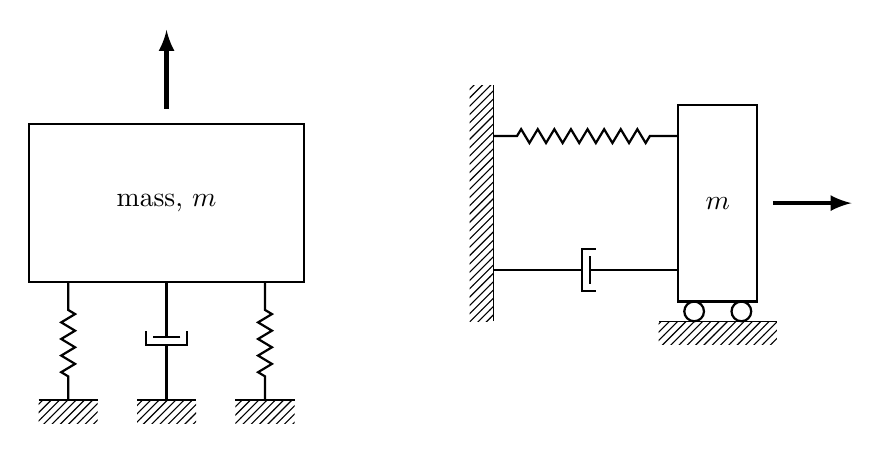
\begin{tikzpicture}[every node/.style={draw,outer sep=0pt,thick}]
\tikzstyle{spring}=[thick,decorate,decoration={zigzag,pre length=0.3cm,post length=0.3cm,segment length=6}]
\tikzstyle{damper}=[thick,decoration={markings,
  mark connection node=dmp,
  mark=at position 0.5 with
  {
    \node (dmp) [thick,inner sep=0pt,transform shape,rotate=-90,minimum width=15pt,minimum height=3pt,draw=none] {};
    \draw [thick] ($(dmp.north east)+(2pt,0)$) -- (dmp.south east) -- (dmp.south west) -- ($(dmp.north west)+(2pt,0)$);
    \draw [thick] ($(dmp.north)+(0,-5pt)$) -- ($(dmp.north)+(0,5pt)$);
  }
}, decorate]
\tikzstyle{ground}=[fill,pattern=north east lines,draw=none,minimum width=0.75cm,minimum height=0.3cm]


\node (M) [minimum width=3.5cm,minimum height=2cm] {mass, $m$};

\node (ground1) at (M.south) [ground,yshift=-1.5cm,xshift=-1.25cm,anchor=north] {};
\draw (ground1.north west) -- (ground1.north east);
\draw [spring] (ground1.north) -- ($(M.south east)!(ground1.north)!(M.south west)$);

\node (ground2) at (M.south) [ground,yshift=-1.5cm,anchor=north] {};
\draw (ground2.north west) -- (ground2.north east);
\draw [damper] (ground2.north) -- ($(M.south east)!(ground2.north)!(M.south west)$);

\node (ground3) at (M.south) [ground,yshift=-1.5cm,xshift=1.25cm,anchor=north] {};
\draw (ground3.north west) -- (ground3.north east);
\draw [spring] (ground3.north) -- ($(M.south east)!(ground3.north)!(M.south west)$);

\draw [-latex,ultra thick] (M.north) ++(0,0.2cm) -- +(0,1cm);

\begin{scope}[xshift=7cm]
\node (M) [minimum width=1cm, minimum height=2.5cm] {$m$};

\node (ground) [ground,anchor=north,yshift=-0.25cm,minimum width=1.5cm] at (M.south) {};
\draw (ground.north east) -- (ground.north west);
\draw [thick] (M.south west) ++ (0.2cm,-0.125cm) circle (0.125cm)  (M.south east) ++ (-0.2cm,-0.125cm) circle (0.125cm);

\node (wall) [ground, rotate=-90, minimum width=3cm,yshift=-3cm] {};
\draw (wall.north east) -- (wall.north west);

\draw [spring] (wall.170) -- ($(M.north west)!(wall.170)!(M.south west)$);
\draw [damper] (wall.10) -- ($(M.north west)!(wall.10)!(M.south west)$);

\draw [-latex,ultra thick] (M.east) ++ (0.2cm,0) -- +(1cm,0);
\end{scope}
\end{tikzpicture}

\section{Begrüßung ist langweilig}
\label{sec-1}
\section{Begrüßung2 ist auch langweilig}
\label{sec-2}
\section{Moodle}
\label{sec-3}
Passwort: F=ma
\section{Klausur}
\label{sec-4}
11.02.2017 (9 Uhr)
60\% Übungspunkte
\section{Bücher}
\label{sec-5}
\begin{center}
\begin{tabular}{ll}
Buch & Bemerkung\\
\hline
Heintze; Lehrbuch zur Experimentalphysik I & \\
Haliday, Resnick, Walker; Physik & \\
Tipler, Allen; Physik & \\
Demtröder; Experimentalphysik I & \\
Bergman & \\
\end{tabular}
\end{center}

online\ldots{}
\section{Einleitung}
\label{sec-6}
\subsection{Eigenschaften der Physik}
\label{sec-6-1}
Physik ist \uline{nicht} axiomatisch!
\begin{itemize}
\item Nicht alle Gesetze der Natur sind bekannt.
\item Die bekannten Naturgesezte sind \uline{nicht} unumstößlich
\item unfertig
\item empirisch
\item quantitativ
\item experimentell
\item überprüfbar
\item braucht Mathematik
\item Gefühl für Größenordnungen und rationale Zusammenhänge
\end{itemize}
\subsubsection{Beispiel}
\label{sec-6-1-1}
Fermi-Probleme:
\begin{itemize}
\item Anzahl der Klabirstimmer in Chicago?
\item Anzahl der Autos in einem 10km Stau?
\item Anzahl von Fischen im Ozean
\end{itemize}

\subsection{Maßeinheiten}
\label{sec-6-2}
Internationales Einheitensystem (SI)
\subsubsection{Basisgrößen}
\label{sec-6-2-1}
\begin{center}
\begin{tabular}{lll}
Größe & Einheit & Symbol\\
\hline
Länge & Meter & $\si{\meter}$\\
Masse & Kilogramm & $\si{\kg}$\\
Zeit & Sekunden & $\si{\second}$\\
\end{tabular}
\end{center}
\begin{enumerate}
\item Meter
\label{sec-6-2-1-1}
Strecke, die das Lich im Cakuum während der Dauer von $\frac{1}{299792458}\si{\second}$ durchläuft.
\item Sekunde
\label{sec-6-2-1-2}
Das $\SI{9192631770}{}$-fache  der Periodendauder der am Übergang zwischen den beiden Hyperfeinstukturniveaus des Grundzustandes von Atomen des Nukulids $Cs_{133}$ entsprechenden Strahlung.
\item Kilogramm
\label{sec-6-2-1-3}
Das Kilogramm ist die Einheit der Masse, es ist gleich der Masse des internationalen Kilogrammprototyps (ist scheiße).
\begin{enumerate}
\item Avogadroprojekt
\label{sec-6-2-1-3-1}
\[N_A = \frac{M V n}{m}\]
$N_A$: Avogardokonstante ($N_A = \SI{6.0221415e23}{}$)
\end{enumerate}
\end{enumerate}
\subsubsection{Weitere Größen}
\label{sec-6-2-2}
\begin{center}
\begin{tabular}{lll}
Größe & Einheit & Symbol\\
\hline
Strom & Ampere & $\si{\ampere}$\\
Temperatur & Kelvin & $\si{\kelvin}$\\
Lichtstärke & Candla & $\si{\candela}$\\
\end{tabular}
\end{center}

\section{Mechanik}
\label{sec-7}
Kinematik: Beschreibung der Bewegung
Dynamik: Ursache der Berwegung

\subsection{Kinematik des Massenpunktes}
\label{sec-7-1}
\subsubsection{Eindimensionale Bewegung}
\label{sec-7-1-1}
\begin{enumerate}
\item {\bfseries\sffamily TODO} Skizze 1
\label{sec-7-1-1-1}
$x_1,t_1 \longrightarrow x_2, t_2$
Geschwindigkeit
\[v = \frac{\text{Weg}}{\text{Zeit}} = \frac{x_2 - x_1}{t_2 - t_1} = \frac{\Delta x}{\Delta t}\quad [v] = \si{\meter\per\second}~\text{abgeleitete Größe}\]
\item Momentangeschwindigkeit
\label{sec-7-1-1-2}
\[v := \lim_{\Delta t\to 0} \frac{\Delta{x}}{\Delta t} = \frac{\mathrm{d}x}{\mathrm{d}t} = \dot{x}\]
\item Beschleunigung
\label{sec-7-1-1-3}
\[a := \lim_{\Delta t\to 0} \frac{\Delta{v}}{\Delta{t}} = \frac{\mathrm{d}v}{\mathrm{d}t} = \frac{\mathrm{d}^2x}{\mathrm{d}t^2} = \ddot{x}\quad [a]=\si{\meter\per\second\squared}\]
\item Freier Fall
\label{sec-7-1-1-4}
$a = \text{const.}$ (Behauptung)
\[a=\ddot{x} = \text{const} = \dot{v}\]
\$$\rightarrow$§ Integration: \[v(t) = \int_0^t a\mathrm{d}t + v_0 = a t + v_0\]
\[x(t) = x_0 + \int_0^t v(t)\mathrm{d}t = x_0 + \int_0^t (a t + v_0)\mathrm{d}t = \frac{1}{2}a t^2 + v_0 t + x_0\]
Bei unserem Fallturm
\[x(t) = \frac{1}{2}a t^2 \rightarrow a = \frac{2 x}{t^2}\]
\begin{center}
\begin{tabular}{rrr}
$x[\si{\meter}]$ & $t[\si{\milli\second}]$ & $\frac{2x}{t^2}[\si{\meter\per\square\second}]$\\
\hline
0.45 & 304.1 & 9.7321696\\
0.9 & 429.4 & 9.7622163\\
1.35 & 525.5 & 9.7772861\\
1.80 & 606.8 & 9.7771293\\
\end{tabular}
\end{center}
\[x(t) = \frac{1}{2} g t^2,~g=\SI{9.81}{\meter\per\square\second}\]
Die Erdbeschleunigung $g$ ist für alle Körper gleich (Naturgesetz).
\end{enumerate}
\subsubsection{Bewegung im Raum}
\label{sec-7-1-2}
\begin{enumerate}
\item {\bfseries\sffamily TODO} Skizze 2
\label{sec-7-1-2-1}
Ortsvektor:
\[\vec{r}(t) = \begin{pmatrix} x(t) \\ y(t) \\ z(t) \end{pmatrix} = {\begin{pmatrix} x(t) & y(t) & z(t)\end{pmatrix}}^\intercal\]
Durschnittsgeschwindigkeit
\[\frac{\vec{\Delta r_{12}}}{\Delta t} = \frac{\vec{r_2} - \vec{r_1}}{\Delta t} = \vec{v_D}\]
\[\vec{v}(t) = \frac{\mathrm{d}\vec{r}}{\mathrm{d}t} = \dot{\vec{r}}(t) = {\begin{pmatrix}\dot{x}(t) & \dot{y}(t) & \dot{z}(t)\end{pmatrix}}^\intercal = {\begin{pmatrix} v_x & v_y & v_z\end{pmatrix}}^\intercal\]
\[\vec{a}(t) = \frac{\mathrm{d}\vec{v}}{\mathrm{d}t} = \dot{\vec{v}}(t) = \ddot{\vec{r}}(t) = {\begin{pmatrix} \ddot{x} & \ddot{y} & \ddot{z}\end{pmatrix}}^\intercal = {\begin{pmatrix} a_x & a_y & a_z \end{pmatrix}}^\intercal\]
$\rightarrow$ Superpositionsprinzip: \\
    Kinematik kann für jede einzelne (Orts)komponente einzeln betrachtet werden.

\[\vec{a_0} = \text{const}\]
\[\vec{r}(t) = \vec{r_0} + \vec{v_0}(t-t_0) + \frac{1}{2}\vec{a}(t^2-t_0^2) = \begin{pmatrix} x_0 + v_{x,0}(t-t_0) + \frac{1}{2} a_{x,0}(t^2-t_0^2) \\ y_0 + v_{y,0}(t-t_0) + \frac{1}{2} a_{y,0}(t^2-t_0^2) \\ z_0 + v_{z,0}(t-t_0) + \frac{1}{2} a_{z,0}(t^2-t_0^2) \end{pmatrix}\]
\item Horizontaler Wurf
\label{sec-7-1-2-2}
\item {\bfseries\sffamily TODO} Skizze 3
\label{sec-7-1-2-3}
\[t_0 = 0\]
\[\vec{a_0} =  {\begin{pmatrix} 0 & 0 & -g \end{pmatrix}}^\intercal\]
\[\vec{v_0} =  {\begin{pmatrix} v_{x,0} & 0 & 0 \end{pmatrix}}^\intercal\]
\[\vec{x_0} =  {\begin{pmatrix} 0 & 0 & 0 \end{pmatrix}}^\intercal\]
\[\vec{r}(t) =  {\begin{pmatrix} v_{x,0}t & 0 & \frac{1}{2}gt^2 \end{pmatrix}}^\intercal\]

\item Schiefer Wurf
\label{sec-7-1-2-4}
\[\vec{a_0} = \cvec{0;0;-g}\]
\[\vec{v_0} = \cvec{v_{x,0};0;v_{z,0}}\]
\[\vec{r_0} = \cvec{0;0;z_0}\]
\[r(t) = \cvec{v_{x,0}t;0;-\frac{1}{2}gt^2 + v_{z,0}t + z_0}\]
\[z(x) = -\frac{1}{2}\frac{g}{v_{x,0}^2}x^2 + \frac{v_{z,0}}{v_{x,0}}x + z_0\]

\item Nachtrag
\label{sec-7-1-2-5}
\[a = \dot{v}\]
\[\int_0^t \dot{v}\d t' = \int_0^ta\d t'\]
\[v\mid_0^t = at'\mid_0^t\]
\[v(t) - \underbrace{v(0)}_{v_0} = at\]
\[v(t) = at + v_0\]
analog:
\[x(t) = \frac{1}{2}at^2 + v_0 t + x_0\]
\begin{enumerate}
\item {\bfseries\sffamily TODO} Skizze Wurfparabel
\label{sec-7-1-2-5-1}
\[\tan{\varphi} = \frac{v_{z,0}}{v_{x,0}}\]
\[v_0^2 = v_{x,0}^2 + v_{z,0}^2\]
Scheitel:
\[Z'(x_s) = 0\]
\[x_s = \frac{v_0^2}{2g}\sin{2\varphi}\]
Wurfweite:
\[Z(x_w) = 0\]
\[x_w = \frac{v_0^2}{2g}\sin{2\varphi}(1 + \sqrt{1 + \frac{2gz_0}{v_0^2\sin^2{\varphi}}})\]
Optimaler Winkel: $\varphi_{opt}, x_w$ max.
\[z_0 = 0\Rightarrow \sin{2\varphi} = 1 \rightarrow \varphi = \SI{45}{\degree}\]
\[z_0 \neq 0\Rightarrow \sin{\varphi_{opt}} = (2 + \frac{2gz_0}{v_0^2})^{-\frac{1}{2}}\]
\end{enumerate}
\item Gleichförmige Kreisbewegung
\label{sec-7-1-2-6}
\[\vec{r}(t) = \cvec{x(t);y(t)} = \cvec{R\cos{\varphi}; R\sin{\varphi}}\]
mit $\varphi = \varphi(t)$
\[\vec{v}(t) = \cvec{\dot{x};\dot{y}} = \cvec{-R\dot{\varphi}\sin{\varphi};R\dot{\varphi}\cos{\varphi}}\]
Gleichförmige Kreisbewegung: $\dot{\varphi} = \text{const}$
Definition Winkelgeschwindigkeit:
\[\omega = \frac{\d \varphi}{\d t} = \dot{\varphi}\quad[w] = \si{\radian\per\second} = \si{1\per\second}\]
Für $\omega = \text{const.}$:
\[\vec{r} = R\cvec{\cos{\varphi};\sin{\varphi}}~\rightarrow \abs{\vec{r}(t)} = r = \text{const}\]
\[\vec{v} = R\omega\cvec{-\sin{\varphi};\cos{\varphi}}~\rightarrow \abs{\vec{r}(t)} = r = \text{const}\]
\[\vec{v} \perp \vec{r} \Leftrightarrow \vec{v}\cdot\vec{r} = 0\]
\begin{enumerate}
\item {\bfseries\sffamily TODO} Skizze Kreisbewegung
\label{sec-7-1-2-6-1}
\item Mitbewegtes Koordinatensystem
\label{sec-7-1-2-6-2}
\[\vec{r}(t) = R\vec{e_R} \quad \vec{e_R} = \cvec{\cos{\varphi (t)};\sin{\varphi (t)}}\]
\[\vec{v}(t) = R\omega \vec{e_t} \quad \vec{e_t} = \cvec{-\sin{\varphi (t)}; \cos{\varphi (t)}}\]
\[\vec{t} \neq~\text{const das heißt}~\vec{a}(t)\neq 0\]
Kreisbeschleunigung
\[\vec{a}(t) = \cvec{\ddot{x}(t);\ddot{y}(t)} = \cvec{-R\omega^2\cos{\varphi};-R\omega^2\sin{\varphi}} = -R\omega^2\vec{e_R} \Rightarrow \vec{a}  \parallel \vec{r}\]
\[\abs{\vec{a}(t)} = R\omega^2 = \frac{v^2}{R} \neq 0\]
Zentripetalbeschleunigung
Zeigt in Richtung des Ursprungs.
\[\vec{a}_{zp} = -R\omega^2\vec{e_R}\]
\item Allgemein
\label{sec-7-1-2-6-3}
\[\vec{\omega}\]
Räumliche Lage der  Bewegungsebene
\[\vec{v} = \v{w}\times  \v r \quad v = \omega r\]
\[\v a = \v w \times \v v\]
\begin{enumerate}
\item {\bfseries\sffamily TODO} Skizze omega
\label{sec-7-1-2-6-3-1}
\end{enumerate}
\end{enumerate}
\item Allgemeine Krummlinige Bewegung
\label{sec-7-1-2-7}
\[\v v = v \v{e_t}\]
\[\v a = \dot{\v v} = \frac{\d (v\v{e_t})}{\d t} = \frac{\d v}{\d t}\v{e_t} + v\frac{\d v{e_t}}{\d t}\]
\[\v{e_t} = \cos{\rho}\v{e_x} + \sin{\rho}\v{e_y}\]
\[\v{e_n} = -\sin{\rho}\v{e_x} + \cos{\rho}\v{e_y}\]
\[\frac{\d \v{e_t}}{\d t} = \dot\rho -\sin{\rho}\v{e_x} + \cos{\rho}\v{e_y} = \dot\rho \v{e_n}\]
\[\v a = \dot v \v{e_t} + \frac{v^2}{\rho}\v{e_n}\]
\begin{enumerate}
\item {\bfseries\sffamily TODO} Skizze
\label{sec-7-1-2-7-1}
\end{enumerate}
\item Relativbewegung
\label{sec-7-1-2-8}
\begin{itemize}
\item $S$-Laborsystem
\item $S'$-Bewegtes System
\item $\v u = (u, 0, 0) = \text{const}$ Geschwindigkeit von S' im System S
\item Punkt $P=(x,y,z)$ in $S$
\item Punkt $P'=(x',y',z')$ in $S'$
\item Zeitpunkt $t = 0: \quad S=S', P=P'$
\end{itemize}
\begin{enumerate}
\item {\bfseries\sffamily TODO} Skizze Bewegtes Bezugssystem
\label{sec-7-1-2-8-1}
\item Galilei-Transformation
\label{sec-7-1-2-8-2}
\begin{enumerate}
\item Eindimensional
\label{sec-7-1-2-8-2-1}
\[x' = x - ut\]
\[y' = y\]
\[z' = z\]
\[v' = v - u\]
\[t' = t\]
\item Dreidimensional
\label{sec-7-1-2-8-2-2}
\[\v r' = \v r - \v u t\]
\[\v v' = \v v - \v u\]
\[\v a' = \v a\]
\end{enumerate}
\end{enumerate}
\end{enumerate}
\subsection{Newtonsche Dynamik}
\label{sec-7-2}
Warum bewegen sich Körper?\\
   Newton 1686: Ursache von Bewegungsänderungen sind Kräfte.
Newtonsche Gesetze (Axiome)
\begin{enumerate}
\item Jeder Körper verharrt im Zustand der Ruhe oder der gleichförmigen Bewegung, sofern er nicht durch Kräfte gezwungen wird diesen Bewegungszustand zu verlassen
\item Die Änderung einer Bewegung wird durch Einwirken einer Kraft verursacht. Sie geschieht in Richtung der Kraft und ist proportional zu Größe der Kraft
\item Übt ein Körper $1$ auf einen Körper $2$ die Kraft $F_{12}$, so reagiert Körper $2$ auf den Körper $1$ mit der Gegenkraft $F_{21}$ und es gilt $F_{21} = -F_{12}$ (actio = reactio)
\end{enumerate}
\subsubsection{Kraft und Impuls}
\label{sec-7-2-1}
\[\v F = \cvec{F_x;F_y;F_z}\]
Superpositions von Kräften (Zusatz zu den Newtonschen Gesetzen (Korollar)):
\[\v{F}_{\text{ges}} = \sum_{i = 1}^n \v{F_i}\]
\begin{enumerate}
\item {\bfseries\sffamily TODO} Skizze Addition von Kräften
\label{sec-7-2-1-0-1}
\item Grundkräfte der Natur
\label{sec-7-2-1-0-2}
\begin{itemize}
\item Elektromagnetische Kraft
\item Starke Draft
\item Schwache Kraft
\item Gravitation
\end{itemize}
\item Impuls
\label{sec-7-2-1-1}
\[\v P = m\v v\quad [\v P] = \si{\kg\meter\per\second}\]
\item Kraft
\label{sec-7-2-1-2}
\[\v F = \f{\d\v P}{\d t} = \dot{\v P} = \f{\d}{\d t}(m\v v)\]
$m = \text{const.}$:
\[\v F = m \f{\d\v v}{\d t} = m\dot{\v v} = m\ddot{\v x} = m\v a\]
\item Grundgesetz der Dynamik
\label{sec-7-2-1-3}
\[\v F = \dot{\v P}~\text{beziehungsweise}~\v F = m\v a\]
\begin{enumerate}
\item Trägheitsprinzip (Impulserhaltung)
\label{sec-7-2-1-3-1}
\[\v P = m\v v = \text{const},~\v P = 0~\text{für}~\v F = 0\]
\end{enumerate}
\item Expermiment
\label{sec-7-2-1-4}
\[\v F_G = \underbrace{m\v g}_{Kraft} = \underbrace{(m + M)}_{Trägheit}\v a = m_{\text{ges}}\v a\]
\[\v a = \f{m}{m + M}\v g \xLeftrightarrow{d = 1} a = \f{m}{m + M}g = \f{m}{m_{text{ges}}}g\]
\begin{enumerate}
\item Erwartung:
\label{sec-7-2-1-4-1}
$a\sim {\f{m}{m_{\text{ges}}}}$, $a = \f{2\Delta s}{\Delta s}$, weil $\Delta s = \f{1}{2} a\Delta t^2$
\item Messung:
\label{sec-7-2-1-4-2}
\begin{center}
\begin{tabular}{rrrrrrr}
$m[\si{\gram}]$ & $M[\si{\gram}]$ & $m_{\text{ges}}[\si{\gram}]$ & $\f{m_{\text{ges}}}{m}$ & $\Delta s[\si{\mm}]$ & $\Delta t [\si{\second}]$ & $a[\si{meter\per\second}]$\\
\hline
10 & 470 & 480 & 48 & 800 & 2.75 & 0.21157025\\
40 & 440 & 480 & 12 & 800 & 1.40 & 0.81632653\\
10 & 1910 & 1920 & 192 & 800 & 5.55 & 0.051943836\\
40 & 1880 & 1920 & 48 & 800 & 2.79 & 0.20554721\\
\end{tabular}
\end{center}
\item {\bfseries\sffamily TODO} Skizze
\label{sec-7-2-1-4-3}
\end{enumerate}
\item Trägheitsprinzip - "revisited"
\label{sec-7-2-1-5}
\textbf{Definition}: Ein Bezugssystem in dem das Trägheitsprinzip gilt nennt man ein Inatialsystem. \\

In einem beschleunigten Bezugsystem gilt das Trägheitsprinzip \uline{nicht}. Beschleunigte Systeme $\neq$ Inatialsysteme.
Das Trägheitsprinzip ist Galilei-invariant.

\begin{enumerate}
\item {\bfseries\sffamily TODO} Skizze whatever
\label{sec-7-2-1-5-1}
\item Trägheitsprinzip: [moderne Formulierung]:
\label{sec-7-2-1-5-2}
Es gibt Inatialsysteme, das heißt Koordinatensysteme  in denen ein Kräftefreier Körper im Zustand der Ruhe oder der gradlinig gleichförmigen Bewegung verbleibt.
\end{enumerate}

\item Actio gleich Reactio
\label{sec-7-2-1-6}
\[\underbrace{\v{F_{12}}}_{\text{Kraft}} = \underbrace{-\v{F_{21}}}_{\text{Gegenkraft}}\]
\begin{enumerate}
\item {\bfseries\sffamily TODO} Skizze von Körpern
\label{sec-7-2-1-6-1}
\item {\bfseries\sffamily TODO} (Skizze) Expermiment
\label{sec-7-2-1-6-2}
\begin{enumerate}
\item Erwartung:
\label{sec-7-2-1-6-2-1}
\[v_1 = v_2 \rightarrow a_1 = a_2 \rightarrow F_1 = F_2~\checkmark\]
Nichttrivialer Fall: \\
       Kraftstoß: \\
       Magnetische Kraft: $F_{\text{mag}} \sim {\f{1}{r^2}}$
\[v_{1,2} = \int_0^{t_{1,2}} a(t)\d t = a_{\text{eff}}T\]
\[\rightarrow F_1(t) = F_2(t) \rightarrow v_1 = v_2\]
\end{enumerate}
\item Expermiment 2
\label{sec-7-2-1-6-3}
\[m_1 = \SI{241.8}{\gram} \wedge \m_2 = \SI{341.8}{\gram} \Rightarrow \f{m_2}{m_1} \approx 1.5\]
\[v = \f{\Delta s}{\Delta t} \rightarrow \f{v_1}{v_2} = \f{t_2}{t_1} = \f{71}{48} \approx 1.5\]
\[a\sim v, F = m a \rightarrow \f{v_1}{v_2} = \f{a_1}{a_2} = \f{m_2}{m_1}\cdot \f{F_1}{F_2}\]
\[1 = \f{F_1}{F_2} \Rightarrow F_1 = F_2\]
\item Beispiele
\label{sec-7-2-1-6-4}
\begin{itemize}
\item Kraft und Gegenkraft (TODO Skizze)
\item Flaschenzug, Seilkräfte (TODO Skizze)
\end{itemize}
\end{enumerate}
\end{enumerate}

\subsection{{\bfseries\sffamily TODO} Montag}
\label{sec-7-3}
\subsubsection{Normalkraft}
\label{sec-7-3-1}
\begin{enumerate}
\item (Skizze) Normalkraft $\v{F}_N$ = Kraft senktrecht zur Kontaktfläche. Wird kompensiert duchr $\v{F}_N'$ = Kraft mit der die Unterlage auf Körper wirkt (Źwangskräfte)
\end{enumerate}
\subsubsection{Schiefe Ebene}
\label{sec-7-3-2}
\begin{itemize}
\item Gewichtskraft: $\v{F}_G = m\v g$
\item Normalkraft: $\v{F}_N = m g\cos{\alpha} \v{e}_y$
\item Hangabtriebskraft: $\v{F}_H = m g\sin{\alpha} \v{e}_x$
\end{itemize}
Bewegungsgleichung
\[F_H = m\ddot{x} \rightarrow x_x = g\sin{\alpha} =\text{const.}\]
\subsubsection{Reibungskräfte}
\label{sec-7-3-3}
\begin{itemize}
\item im täglichen Leben über all präsent
\item spielt eine wichtige Rolle Technik
\end{itemize}
$\rightarrow$ Tribologie = Reibungslehre
\begin{itemize}
\item Reibung hängt stark von der Oberfläche ab
\end{itemize}
\begin{enumerate}
\item Experiment: Bewegung einer Masse
\label{sec-7-3-3-1}
\begin{itemize}
\item Gewicht ruhte: $\v{F}_Z = - \v{F}_R \to a = 0, v = 0$
\item Gewicht setzt sich in Bewegung: $\abs{\v{F}_Z} > \abs{\v{F}_R} \to a > 0,v$ steigt an
\item Gewicht gleitet: $\v{F}_Z = - \v{R}_R \to a = 0, v =~\text{const.}~\neq 0$ mit $\v v =~\text{const}~$
\end{itemize}
Reibugskraft nimmt ab, sobald das Gewicht bewegt wir.
\begin{itemize}
\item Haftreibung $F_H$ \\
       Schwellenwert für Zugkraft um Körper zu bewegen
\item Gleitreibung $F_G$ \\
       Reibungskreaft bei bewegtem Körper
\end{itemize}

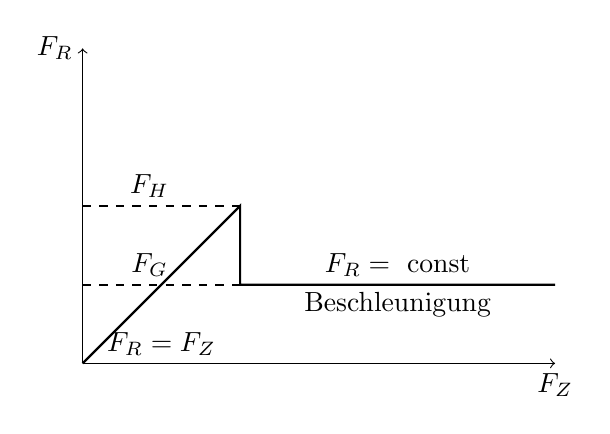
\begin{tikzpicture}

% horizontal axis
\draw[->] (0,0) -- (6,0) node[anchor=north] {$F_Z$};

% vertical axis
\draw[->] (0,0) -- (0,4) node[anchor=east] {$F_R$};

% Us
\draw[thick] (0,0) -- (2,2) -- (2,1) -- (6,1);
\draw (1,0.25) node {$F_R = F_Z$}; %label

\draw[thick,dashed] (0,2) -- (2,2);
\draw (0.85,2.25) node {$F_H$}; %label

\draw[thick,dashed] (0,1) -- (2,1);
\draw (0.85,1.25) node {$F_G$}; %label

\draw (4,1.25) node {$F_R =~\text{const}$};
\draw (4, 0.75) node {Beschleunigung};

\end{tikzpicture}

\item Experiment: Tribologische Messung
\label{sec-7-3-3-2}
Messung der Zugkraft bei der sich der Holzblock nach kleiner Störung in Richtung Rolle bewegt: $F_R = F_Z$
\begin{enumerate}
\item Beobachtung
\label{sec-7-3-3-2-1}
\begin{itemize}
\item $F_R$ hängt nicht von der Oberfläche ab.
\item $F_R$ hängt von dem Gewicht des Blocks ab
\item $F_R$ ist Materialbhängig
\end{itemize}
\end{enumerate}
\end{enumerate}

\subsubsection{Tribologische Reibungslehre}
\label{sec-7-3-4}
\[F_G = \mu_G F_N \tag{$\mu_G=$ Gleitreibungskraft}\]
\[F_H = \mu_H F_H \tag{$\mu_H=$ Haftreibungskraft}\]
\[\mu_H > \mu_G\]
\subsubsection{Mikroskopisches Modell}
\label{sec-7-3-5}
Verantwortlich sind elektrische Kröfte zwischen Atomen und Molekülen der beieinanderliegenden Oberflächen: Van-der-Waals-Kräfte
\begin{itemize}
\item Stärke ergibt sich aus effektivem Kontakt.
\end{itemize}
Relative mikroskopische Reibungsfläche: $\sum \frac{a_i}{A} \sim \frac{F_N}{A} \leftarrow~\text{Druck}$
\begin{itemize}
\item $a_1$ = effektive Kontaktfläche eines Einzelatoms
\end{itemize}
Also: \[F_R \sim \sum \frac{a_i}{A} \sim F_N\]
\begin{itemize}
\item Haftreibung: Verzahnung der Oberflächen mit minimalen Abstand
\item Gleitreibung: Minimaler Abstand wird aufgrund der Bewegung nicht erreicht
\end{itemize}
\subsubsection{Schiefe Ebene: Messung der Reibungskraft (Skizze)}
\label{sec-7-3-6}
Kräftegleichgewicht: $F_H = F_R$
\[F_H = m g \sin{\alpha}, F_N = m g \cos{\alpha}\]
Grenzwinkel: $F_R = m g \sin{\alpha} = \mu_R m g \cos{\alpha} \Rightarrow \mu_R = \tan{\alpha}$
\[\alpha = \SI{15}{\degree} \rightarrow \tan{\alpha} = 0.27,\mu_G = 0.27\]
\subsubsection{Zentripetalkraft}
\label{sec-7-3-7}
\[\v a_{Zp} = \v \omega \times(\v\omega\times\v r)\quad \v{F}_{Zp} = m\v\omega\times(\v\omega\times\v r)\]
\[a_{Zp} = \omega^2 r = \frac{v^2}{r}\quad F_{Zp} = m\omega^2 r = m \frac{v^2}{r}\]
\begin{enumerate}
\item Beispiel 1 Rotierendes Pendel
\label{sec-7-3-7-1}
\[\v{F}_{Zp} := \v{F}_G + \v{F}_Z\]
\[F_G = m g = F_Z \cos{\theta}\]
\[F_{Zp} = F_Z \sin{\theta}\]
\[F_{Zp} = mg \frac{\sin{\theta}}{\cos{\theta}} = m g \tan{\theta},\quad a_{Zp} = g\tan{\theta}\]
\[a_{Zp} = \omega^2 r \Rightarrow: \omega \sqrt{\frac{g}{\tan{\theta}}}\]
\begin{itemize}
\item $\theta$ steigt mit $\omega$ an
\item $\theta(\omega)$ ist unabhängig von Masse
\end{itemize}
\item Beispiel 2 Geostationärer Satellit
\label{sec-7-3-7-2}
Zetripetal = Gravitationskraft \\
     \[m\omega^2 R = G\frac{m M_E}{R^2}\]
Geostationär: $\omega = \frac{2\pi}{\SI{24}{\hour}} = \frac{2\pi}{24\cdot\SI{3600}{\second}} = \SI{7.27e-5}{\per\second}$
\[R^3 = \frac{G M_E}{\omega^2} \rightarrow R = \SI{42312}{\kilo\meter}\]
Abstand von der Erd-Oberfläche: \[\tilde{R} = R - R_E = \SI{35930}{\kilo\meter}\]
\begin{itemize}
\item $G = \SI{6.67e-11}{\meter\cubed\per\kilo\gram\second\squared}$
\item $M_E = \SI{6e24}{\kilo\gram}$
\item $R_E = \SI{6373}{\kilo\meter}$
\end{itemize}
\end{enumerate}
% Emacs 25.1.1 (Org mode 8.2.10)
\end{document}